\question{Câu 6}

 Cho mạch khuếch đại tín hiệu được ghép liên tầng như hình vẽ. Giả sử các tụ có điện dung rất lớn. Các thông số $\beta = 100$,  $K_{n}=1 mA/V^{2}$, $V_{TN} = 1 V$. BJT có $V_{A} = \infty$  và FET có $\lambda = 0$. 
 
 \begin{figure}[H]
 	\centering
 	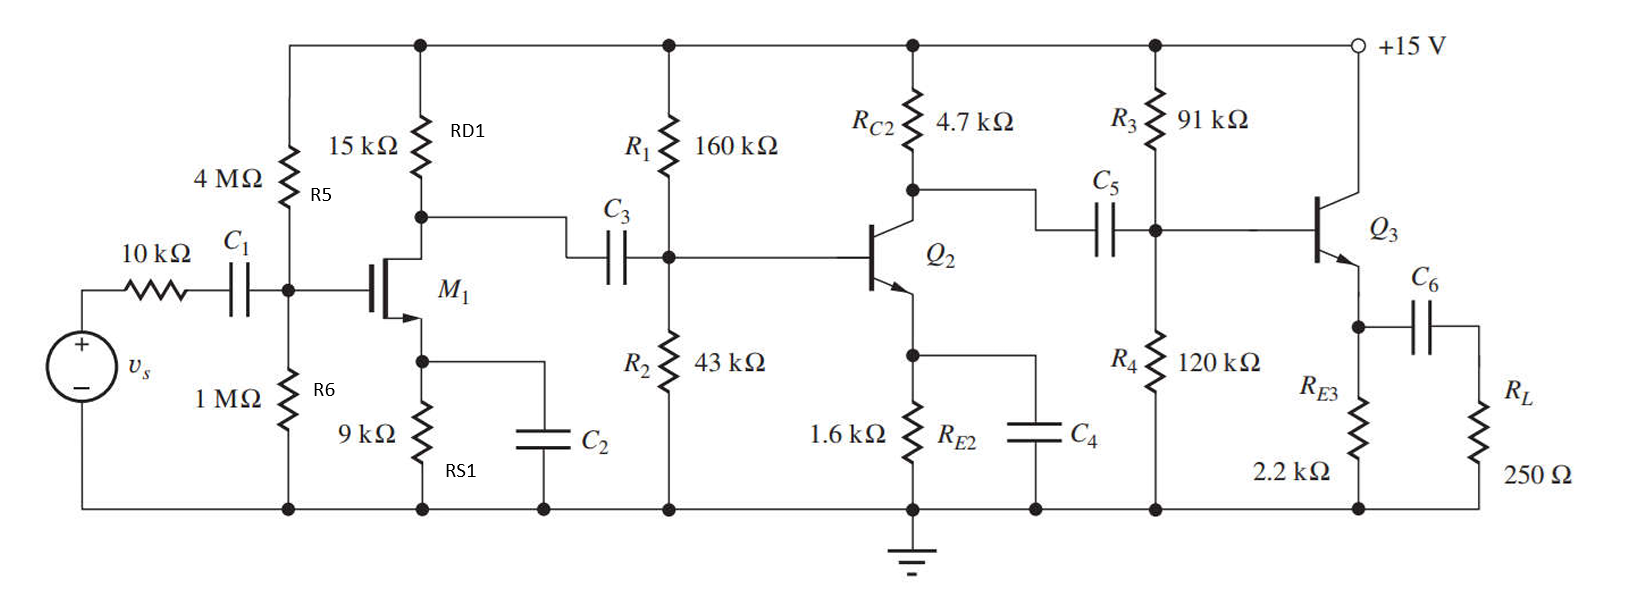
\includegraphics[width=.9\linewidth]{./my-chapters/my-images/Question6/DeBai.png}
 \end{figure}
 
% \begin{enumerate}[label=\alph*)]
% 	\item Tìm điểm hoạt động Q của các transistor.
% \end{enumerate}

\answer{a}{Tìm các điểm hoạt động của Q}

\noindent Xét hoạt động chế độ DC cho toàn mạch.

\begin{itemize}[label=-]

	\item Tầng 1:
	
	\begin{minipage}{0.4\linewidth}
		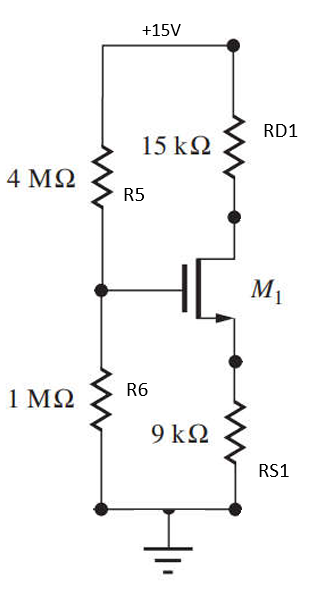
\includegraphics[width=.7\linewidth]{./my-chapters/my-images/Question6/DC_tang1.png}
	\end{minipage}
	\begin{minipage}{0.1\linewidth}
		$\Rightarrow$
	\end{minipage}
	\begin{minipage}{0.4\linewidth}
		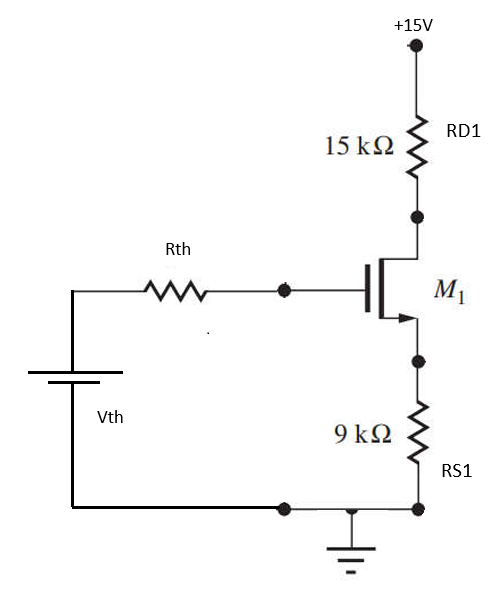
\includegraphics[width=.8\linewidth]{./my-chapters/my-images/Question6/DC_tang1 - Copy.png}
	\end{minipage}
	
	Thevenin ta có:
		\[ R_{th} = R_{5}//R_{6} = \dfrac{4M \times 1M}{4M + 1M} = 0.8M \Omega \]
		\[ V_{th} = \dfrac{R6}{R_{5} + R_{6}}\times V_{cc} = \dfrac{1M}{1M + 4M}\times 15 = 3V\]
		$\Rightarrow V_{G} = 3V \Rightarrow V_{GS} = V_{G} - V_{S} = 3 - V_{S}$
		
		Với $V_{S} = I_{DS} \times R_{S1} \Rightarrow V_{GS} = 3 - I_{DS}\times R_{S1}$
		\[ \begin{matrix}
			I_{DS1} & = & \dfrac{1}{2} K_{n} (V_{GS} - V_{tn})^{2} \hfill \\
			       & = & \dfrac{1}{2} K_{n} (3 - I_{DS}\times R_{S1} - V_{tn})^{2} \hfill \\
			       & = & \dfrac{1}{2} (3 - I_{DS}\times 9 - 1)^{2} \hfill \\ 
		\end{matrix}
		\]
		
		\[ \Rightarrow
		\begin{cases}
			I_{DS1} = 0.3097mA \rightarrow V_{GS} = 3 - 0.3097\times 9 = 0.2127V < V_{tn}(\text{Loại}) \\
			I_{DS1} = 0.1595mA \rightarrow V_{GS} = 3 - 0.1595\times 9 = 1.5645V > V_{tn}(\text{Thỏa})
		\end{cases}\]
		$ \Rightarrow V_{D} = V_{cc} - I_{D} \times R_{D1} = 15 - 0.1595\times 15 = 12.6075V $
		
		$ \Rightarrow V_{DS1} = V_{D} - V_{S} = 11.1720V $
		
		Vậy điểm làm việc Q của tâng 1 là : $(I_{DS1}, V_{DS1}) = (0.1595mA, 11.1720V)$.
		
		\item Tầng 2:
		
		\begin{minipage}{0.4\linewidth}
			\includegraphics[width=.7\linewidth]{./my-chapters/my-images/Question6/DC_tang2.png}
		\end{minipage}
		\begin{minipage}{0.1\linewidth}
			$\Rightarrow$
		\end{minipage}
		\begin{minipage}{0.4\linewidth}
			\includegraphics[width=.8\linewidth]{./my-chapters/my-images/Question6/DC_tang2 - Copy.png}
		\end{minipage}
		
			Thevenin ta có:
		\[ R_{th} = R_{1}//R_{2} = \dfrac{160k \times 43k}{160k + 43k} \approx 33.8916k \Omega \]
		\[ V_{th} = \dfrac{R2}{R_{1} + R_{2}}\times V_{cc} = \dfrac{43k}{160k + 43k}\times 15 \approx 3.1773V\]
		
		Áp dụng KVL cho vòng (1):
		\[ -I_{E2}\times R_{E2} - V_{BE} - I_{B2}\times R_{th} + V_{th} = 0 \]
		Ta có: $I_{E2} = (\beta + 1) I_{B}$
		\[ \Rightarrow I_{B} = \dfrac{V_{th} - V_{BE}}{R_{th} + (\beta + 1)R_{E2}} = \dfrac{3.1773 - 0.7}{33.8916 + (100+1)1.6} = 0.0127mA\]
		Ta có: $I_{C2} = \beta I_{B2} = 100\times 0.0127mA = 1.270mA$.
		
		Áp dụng KVL cho vòng (2):
		\[-V_{cc} + I_{C2}R_{C2} + V_{CE} + I_{E2}R_{E2} = 0 \]
		Ta có: $I_{C2} = \dfrac{\beta}{\beta + 1}I_{E2} = \alpha I_{E2} \approx I_{E2}$
		
		\[ \Rightarrow V_{CE2} = V_{cc} - I_{C2}(R_{C2} + R_{E2}) = 15 - 1.270(4.7 + 1.6) = 6.9990V\]
		
		Vậy điểm làm việc Q của tâng 2 là : $(I_{CQ2}, V_{CEQ2}) = (1.270mA, 6.9990V)$.
		
		\item Tầng 3:
		
		\begin{minipage}{0.4\linewidth}
			\includegraphics[width=.7\linewidth]{./my-chapters/my-images/Question6/DC_tang3.png}
		\end{minipage}
		\begin{minipage}{0.1\linewidth}
			$\Rightarrow$
		\end{minipage}
		\begin{minipage}{0.4\linewidth}
			\includegraphics[width=.8\linewidth]{./my-chapters/my-images/Question6/DC_tang3 - Copy.png}
		\end{minipage}
		
		Thevenin ta có:
		\[ R_{th} = R_{3}//R_{4} = \dfrac{91k \times 120k}{91k + 120k} \approx 51.7536k \Omega \]
		\[ V_{th} = \dfrac{R4}{R_{3} + R_{4}}\times V_{cc} = \dfrac{120k}{91k + 120k}\times 15 \approx 8.5308V\]
		
		Áp dụng KVL cho vòng (1):
		\[ -I_{E3}\times R_{E3} - V_{BE} - I_{B3}\times R_{th} + V_{th} = 0 \]
		Ta có: $I_{E3} = (\beta + 1) I_{B3}$
		\[ \Rightarrow I_{B3} = \dfrac{V_{th} - V_{BE}}{R_{th} + (\beta + 1)R_{E3}} = \dfrac{8.5308 - 0.7}{51.7536 + (100+1)2.2} = 0.0286mA\]
		Ta có: $I_{C3} = \beta I_{B3} = 100\times 0.0286mA = 2.86mA$.
		
		Áp dụng KVL cho vòng (2):
		\[-V_{cc} + V_{CE} + I_{E}R_{E2} = 0 \]
		Ta có: $I_{C3} = \dfrac{\beta}{\beta + 1}I_{E3} = \alpha I_{E3} \approx I_{E}$
		
		\[ \Rightarrow V_{CE3} = V_{cc} + R_{E2}I_{E3} = 15 - 2.86(2.2) = 8.708V\]
		
		Vậy điểm làm việc Q của tâng 3 là : $(I_{CQ3}, V_{CEQ3}) = (2.86mA, 8.708V)$.
\end{itemize}

\answer{b}{Tìm $A_{v}$, $G_{v}$, $R_{i}$, $R_{o}$ của mạch.}

\noindent Xét hoạt động chế độ AC cho toàn mạch, ta có mạch tương đương như sau:

\begin{figure}[H]
	\centering
	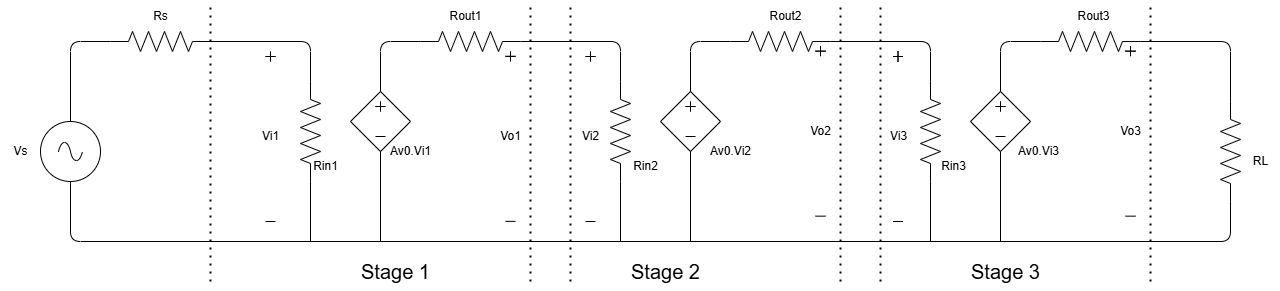
\includegraphics[width=.9\linewidth]{./my-chapters/my-diagrams/Question6/caub_tongquat.png}
\end{figure}

\begin{itemize}[label=-]
	\item Tầng 1:
	
	\begin{figure}[H]
		\centering
		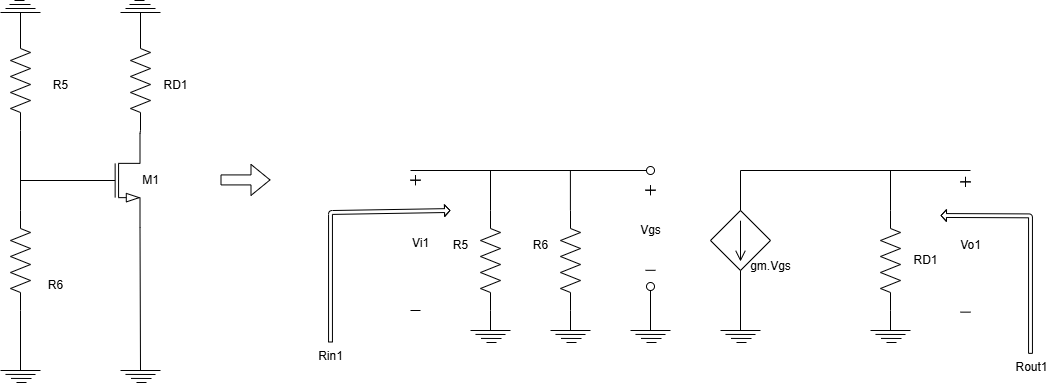
\includegraphics[width=.7\linewidth]{./my-chapters/my-diagrams/Question6/caub_stage1.png}
	\end{figure}
	
	\begin{itemize}[label = +]
		\item $R_{in1} = R_{5} // R_{6} = \dfrac{4M \times 1M}{4M + 1M} = 0.8M \Omega$
		\item $R_{out1} = R_{D1} = 15k \Omega$
		\item $A_{vo_{1}} = \dfrac{v_{o_{1}}}{v_{i_{1}}}|_{R_{L} = \infty} = \dfrac{v_{o_{1}}}{V_{gs}} = -g_{m} R_{D1}$
		
		Trong đó, $g_{m} = \dfrac{2I_{DQ}}{V_{OV}} = \dfrac{2I_{DQ}}{V_{GS} - V_{tn}} = \dfrac{2\times 0.1595mA}{1.5645V - 1V} \approx 0.5651 mA/V$
		
		$\Rightarrow A_{vo_{1}} = -0.5651 mA/V \times 15k = -8.4765 V/V $.
	\end{itemize}
	
	\item Tầng 2:
	
	\begin{figure}[H]
		\centering
		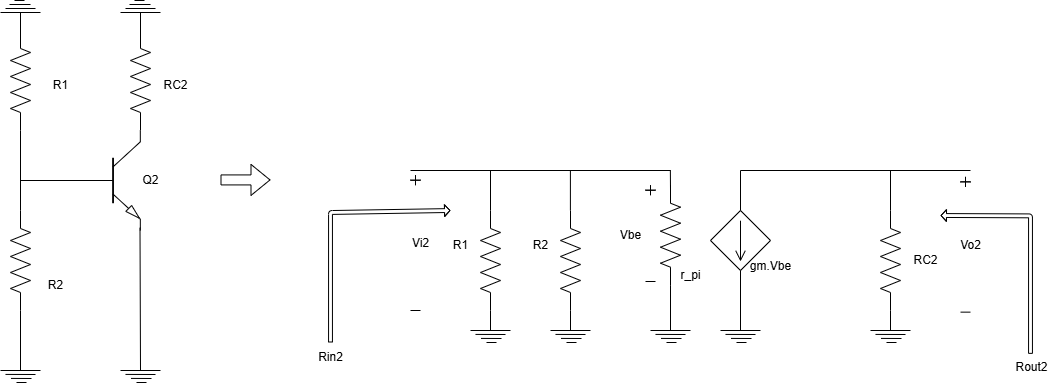
\includegraphics[width=.7\linewidth]{./my-chapters/my-diagrams/Question6/caub_stage2.png}
	\end{figure}
	
	\begin{itemize}[label = +]
		\item $R_{in2} = R_{1} // R_{2} // r_{\pi}$
		
		Trong đó, $r_{\pi} = \dfrac{\beta}{g_{m}} = \beta \dfrac{V_{T}}{I_{C}} = 100 \dfrac{25mV}{1.270mA} = 1.9685k\Omega$
		
		$\Rightarrow R_{in2} = 1.8604k\Omega$
		\item $R_{out1} = R_{C2} = 4.7k \Omega$
		\item $A_{vo_{2}} = \dfrac{v_{o_{2}}}{v_{i_{2}}}|_{R_{L} = \infty} = \dfrac{v_{o_{2}}}{v_{be}} = -g_{m}R_{C2}$
		
		Trong đó, $g_{m} = \dfrac{I_{C}}{V_{T}} = \dfrac{1.270mA}{25mV} = 0.0508 A/V$
		
		$\Rightarrow A_{v_{o_{2}}} = -0.0508\times 4.7k = -238.76 V/V$.
	\end{itemize}
\end{itemize}